\subsection{Deep-Learning Controller}


\subsubsection{Model Architectures}
A number of model architectures were trained in a coarse to fine grid sweep to determine an optimal learning model baseline for future experiments. A summary of the trial results is displayed in Table \ref{tab:arch_search}. Only the best architecture from each trial is shown. For a full breakdown of each trial, see Appendix \ref{app:learning}. In many trials a clear winner is not found, and changing the parameter has little to no effect on the model performance. In these cases, the baseline model selection criteria favours smaller parameters to enable faster run times. 

\begin{table}[h]
    \centering
    \caption{Model architecture search trial summary}
    \makebox[\textwidth][c]{\begin{tabular}{p{0.32\linewidth} | p{0.15\linewidth} | p{0.15\linewidth} | p{0.12\linewidth} | p{0.16\linewidth}  }
        \textbf{Trial Type} & \textbf{Backbone Linear Layer Size(s)} & \textbf{Head Linear Layer Size(s)} & \textbf{LSTM Layer Size} & \textbf{Best RMSE Validation Loss [A]} \\
        \hline
        LSTM layer size search & 10, 10 & 50 & 15 & 0.0220 \\
        Head layer size search & 10, 10 & 0 & 20 & 0.0226 \\
        Head layer depth search & 10, 10 & 25, 25 & 20 & 0.0224 \\
        Backbone layer size search & 30 & 25, 25 & 20 & 0.0205 \\
        Backbone layer depth search & 20, 20 & 25, 25 & 15 & 0.0221 \\
    \end{tabular}}
    \label{tab:arch_search}
\end{table}

The baseline configuration chosen for future trials contains a backbone with two fully connected layers of 10 nodes each, an LSTM state estimator with 30 nodes, and a single fully connected head layer with 100 nodes. Other baseline parameters include: 512 batch size, 1000 epochs, 0.001 learning rate, a \SI{0.2}{s} feedback horizon, and a \SI{0.2}{s} prediction horizon. 

\subsubsection{Feedback Horizon}
Figure \ref{fig:feedback_horizon} shows the model search for an optimal feedback horizon length. The model used for this trial is the baseline model described in Section \ref{sec:learning_baseline_description}. The feedback horizon was varied from \SI{0}{s} (no feedback data is provided) to \SI{15}{s}. The best validation loss achieved from a model trained using each given feedback horizon is presented. 

\begin{figure}[h]
    \centering
    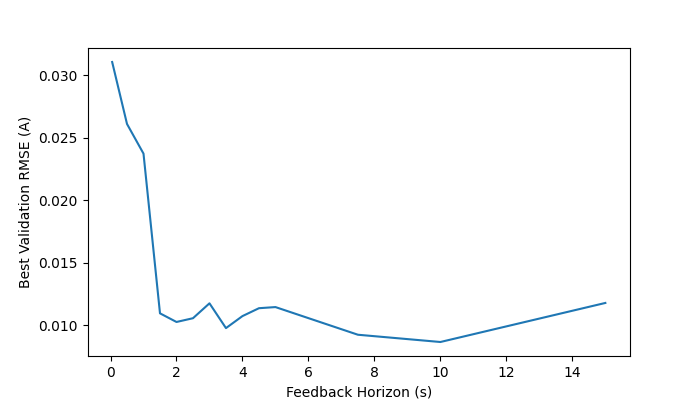
\includegraphics[width=0.75\textwidth]{images/feedback_horizon.png}
    \caption{Best validation losses in feedback horizon trial}
    \label{fig:feedback_horizon}
\end{figure}


\subsubsection{Configuration Parameters}
Figure \ref{fig:configuration_size} shows the model search for an optimal configuration parameter size. The model used for this trial is the baseline model described in Section \ref{sec:learning_baseline_description}. The configuration parameter size was varied from 0 (no configuration parameter is provided) to 20. The configuration parameter size refers to a set of tunable values passed as an input to the model where each set of values is unique to the robot configuration that the data was collected on. Each time the robot broke, a new configuration is labelled.

\begin{figure}[h]
    \centering
    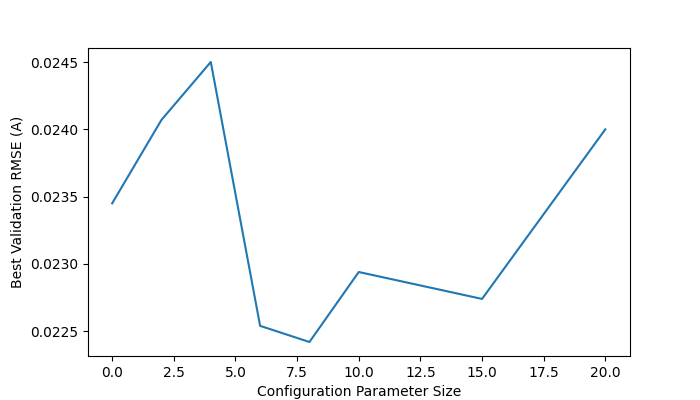
\includegraphics[width=0.75\textwidth]{images/configuration_size.png}
    \caption{Best validation losses in configuration parameter trial}
    \label{fig:configuration_size}
\end{figure}


\subsubsection{Data Weighting}
The data weighing trial compared model performance when trained using weighted prediction labels. Three weight distributions were tested alongside an unweighted baseline. Each weight function was trained with six different model architectures. The results of this trial are shown in Figure \ref{fig:prediction_weighting}. The weight for each trials are sampled from a continuous function defined on the prediction interval. Each set of weights is normalized so that the sum of all weights equals one. The functions used are defined in Table \ref{tab:weights}.

\begin{table}[h]
    \centering
    \caption{Data weight definitions for data weighing trial}
    \makebox[\textwidth][c]{\begin{tabular}{c | c | c}
        \textbf{Weight Class} & \textbf{Function (Pre-Normalization)} & \textbf{Interval}\\
        \hline
        Unweighted & $f(t) = 1$ & N/A\\
        Linear & $f(t) = \frac{t}{3}$ & $[1, 3)$ \\
        Exponential & $f(t) = e^t$ & $[0, 2)$\\
        Quadratic & $f(t) = t^2 - 1.5t + 1.5$ & $[0, 2)$
    \end{tabular}}
    \label{tab:weights}
\end{table}
    
\begin{figure}[h]
    \centering
    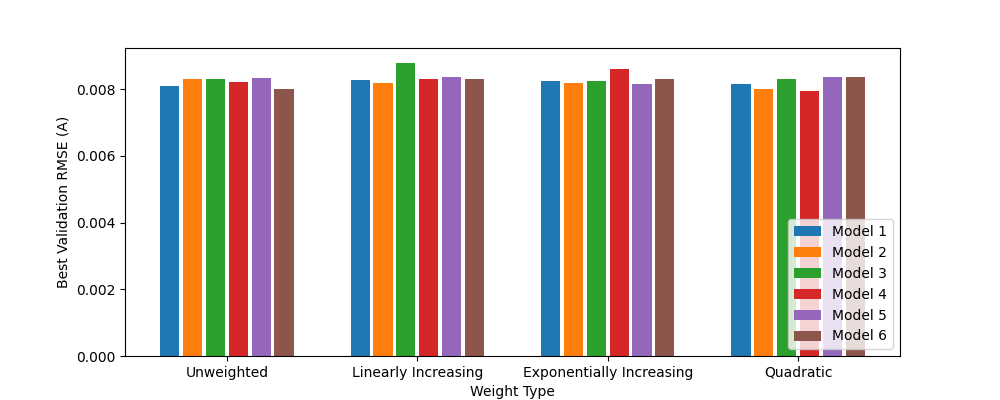
\includegraphics[width=0.95\textwidth]{images/prediction_weighting.png}
    \caption{Best validation losses in prediction weighting trial}
    \label{fig:prediction_weighting}
\end{figure}